% =====================================================================
%  Fundamentals of Deep Learning — Class 6
%  Topic (course plan): Single-layer NN/Shallow NN
%  Subtopics (course plan): Regression and Classification
%  This class: the classification half.  Regression was Class 5.
%
%  Figures: generated by src/build_all.py (one module per figure).
%  Notation: the fixed course convention (see _shared/NOTATION.md) —
%    x features, y targets, yhat predictions, w for every learnable
%    parameter, phi_j RESERVED for fixed basis functions,
%    a pre-activations, z = h(a) hidden units, C_k classes.
%
%  Compile:  xelatex main.tex   (run twice)
% =====================================================================

\documentclass[aspectratio=169, 11pt]{beamer}

\usetheme{metropoliscustom}

\usepackage{graphicx}
\DeclareGraphicsExtensions{.pdf,.png,.jpg}
\graphicspath{{figs/}{Class06_Shallow_NN_Classification/B_Recreated_Figures/figs/}}
\usepackage{amsmath, amssymb}
\usepackage{bm}
\usepackage{tikz}
\usetikzlibrary{arrows.meta, positioning, calc}
\tcbuselibrary{skins}

\definecolor{mlc}{HTML}{341651}    % ML side (indigo)
\definecolor{nnc}{HTML}{800000}    % NN side (maroon)
\definecolor{tealc}{HTML}{1C7293}
\definecolor{shc}{HTML}{341651}
\definecolor{dpc}{HTML}{800000}
\definecolor{accc}{HTML}{B8860B}

% ---- theorem environments -------------------------------------------
\setbeamertemplate{theorems}[numbered]
\newtheorem{lemmax}[theorem]{Lemma}
\newtheorem{propx}[theorem]{Proposition}

% ---- parallel-teaching strip: split box, ML left / NN right ----------
\newcommand{\mlparallel}[2]{%
  \vfill
  {\scriptsize
  \begin{tcolorbox}[enhanced, sidebyside, sidebyside align=top,
                    lefthand ratio=0.485,
                    segmentation style={mlc!35, line width=0.6pt},
                    colback=mlc!5, colframe=mlc!35, boxrule=0.5pt,
                    arc=1.2mm, left=1.6mm, right=1.6mm,
                    top=0.6mm, bottom=0.6mm,
                    before skip=0pt, after skip=0pt]
    {\color{mlc}\textbf{ML}}\hspace{0.55em}#1
  \tcblower
    {\color{nnc}\textbf{NN}}\hspace{0.55em}#2
  \end{tcolorbox}}%
  \vspace{0.35em}%
}

\newcommand{\figsource}[1]{{\scriptsize\color{mcMuted} #1}}
\newcommand{\figcap}[2][0.90]{%
  \begin{center}\begin{minipage}{#1\textwidth}\centering
    {\scriptsize\color{mcMuted} #2}
  \end{minipage}\end{center}}

% =====================================================================
\title{Single-layer NN/Shallow NN}
\subtitle{Regression and Classification}
\author{Fundamentals of Deep Learning \ \textperiodcentered\ Class 6
        \ \textperiodcentered\ Classification}
\institute{}
\date{4 August}

\footleft{Fundamentals of Deep Learning}
\footright{Single-layer NN/Shallow NN}
\titlelogos{}

\begin{document}

\maketitle

\begin{frame}{Outline}
  \tableofcontents
\end{frame}

% =====================================================================
\section{From Regression to Classification}
% =====================================================================

\begin{frame}{Notation used throughout this course}
  \vspace{0.2em}
  {\footnotesize
  \renewcommand{\arraystretch}{1.22}
  \begin{columns}[T, onlytextwidth]
    \begin{column}{0.49\textwidth}
      \begin{tabular}{@{}l@{\hspace{1.5em}}l@{}}
        $\mathbf{x}\in\mathbb{R}^{D}$ & input / \alert{features}\\
        $y$, $\mathbf{y}$ & \alert{target}, targets\\
        $\hat y(\mathbf{x},\mathbf{w})$ & model \alert{prediction}\\
        $\mathcal{C}_1,\dots,\mathcal{C}_K$ & the classes\\
        $N$, $D$, $M$, $K$ & examples, inputs, units, classes\\
        $\mathbf{w}$, $w_0$ & weights, bias\\
      \end{tabular}
    \end{column}
    \begin{column}{0.49\textwidth}
      \begin{tabular}{@{}l@{\hspace{1.5em}}l@{}}
        $\phi_j(\mathbf{x})$ & \alert{fixed} basis function\\
        $a$, $a_k$ & output pre-activation\\
        $z_j=h(a_j)$ & hidden unit\\
        $\sigma(a)$ & logistic sigmoid\\
        $E(\mathbf{w})$ & error function\\
        $\delta_{kj}$ & Kronecker delta\\
      \end{tabular}
    \end{column}
  \end{columns}}
  \vfill
  \begin{redhighlight}
    {\footnotesize Symbols follow \textbf{Bishop \& Bishop (2024)},
    except that targets are written $y$ and predictions $\hat y$.
    For $K$ classes the target is \alert{one-hot}: $y_{nk}\in\{0,1\}$
    with $\sum_k y_{nk}=1$.}
  \end{redhighlight}
\end{frame}

\begin{frame}{What changes, and what does not}
  \centering
  \renewcommand{\arraystretch}{1.25}
  {\small
  \begin{tabular}{p{0.20\textwidth} p{0.33\textwidth}
                  p{0.35\textwidth}}
    & \textbf{\color{mlc}Regression (Class 5)}
    & \textbf{\color{nnc}Classification (today)}\\
    \hline
    Target & $y\in\mathbb{R}$
      & $y\in\{0,1\}$, or one of $K$ classes\\
    Output activation & identity
      & \alert{sigmoid} / \alert{softmax}\\
    Error & sum of squares
      & \alert{cross-entropy}\\
    Prediction & a value
      & a \alert{probability}\\
    \hline
  \end{tabular}}
  \vspace{0.7em}

  {\small The hidden layer is \alert{unchanged}: same architecture,
  same learned features $z_j=h(a_j)$. Only the last step differs.}
  \mlparallel{linear regression $\to$ logistic regression}
             {NN regression $\to$ NN classification, same translation}
\end{frame}

\begin{frame}{Recap: the shallow network}
  \vspace{0.2em}
  From Class~5 (Bishop \& Bishop, 2024, Eqs.~6.1--6.3):
  \[
    a_j = \sum_{i=1}^{D} w_{ji}^{(1)} x_i + w_{j0}^{(1)},
    \qquad
    z_j = h(a_j),
    \qquad
    a_k = \sum_{j=1}^{M} w_{kj}^{(2)} z_j + w_{k0}^{(2)}
  \]
  \vfill
  \begin{itemize}\setlength{\itemsep}{4pt}
    \item {\small Regression: $\hat y_k = a_k$ --- the output
          \emph{is} the pre-activation}
    \item {\small Classification: pass $a_k$ through an
          \alert{output activation} that turns it into a
          probability}
    \item {\small Everything before that last step is identical}
  \end{itemize}
  \mlparallel{$\sigma(\mathbf{w}^{\!\top}
              \boldsymbol{\phi}(\mathbf{x}))$: fixed features}
             {$\sigma(\sum_j w^{(2)}_{j}z_j+w^{(2)}_0)$: learned
              features}
\end{frame}

% =====================================================================
\section{Linear Classifiers and Decision Boundaries}
% =====================================================================

\begin{frame}{Discriminant functions}
  \begin{columns}[T, onlytextwidth]
    \begin{column}{0.46\textwidth}
      \vspace{0.4em}
      {\small The simplest classifier
      (B\&B, 2024, \S5.1.1):}
      \vspace{0.2em}
      \[
        a(\mathbf{x}) = \mathbf{w}^{\!\top}\mathbf{x} + w_0
      \]
      \vspace{0.2em}
      {\small
      \begin{itemize}\setlength{\itemsep}{5pt}
        \item Assign $\mathcal{C}_2$ if $a(\mathbf{x})\ge 0$,
              else $\mathcal{C}_1$
        \item The boundary $a(\mathbf{x})=0$ is a
              \alert{hyperplane}
        \item $\mathbf{w}$ fixes its \alert{orientation},
              $w_0$ its \alert{offset}
      \end{itemize}}
    \end{column}
    \hfill
    \begin{column}{0.50\textwidth}
      \centering
      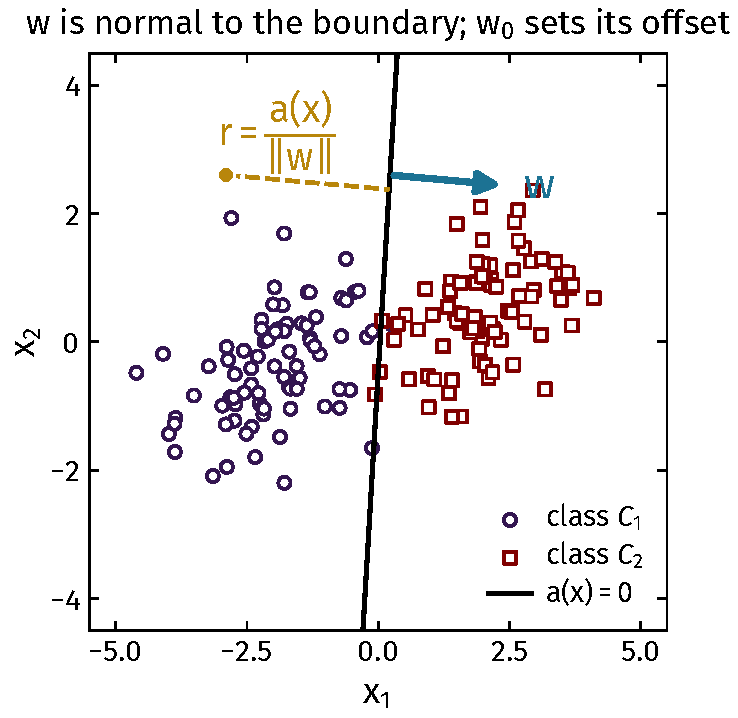
\includegraphics[height=0.375\textheight]{discriminant}
      \\[0.2em]
      \figsource{Two Gaussian classes and the fitted boundary.}
    \end{column}
  \end{columns}
  \vspace{0.75em}
  \mlparallel{a hyperplane in input space}
             {a hyperplane in \emph{learned feature} space}
\end{frame}

\begin{frame}{How far is a point from the boundary?}
  \begin{theorem}[Signed distance to a hyperplane]
    {\small For the hyperplane $a(\mathbf{x})
    =\mathbf{w}^{\!\top}\mathbf{x}+w_0=0$, the signed
    perpendicular distance from any point $\mathbf{x}$ is
    \[
      r \;=\; \frac{a(\mathbf{x})}{\lVert\mathbf{w}\rVert}
      \;=\;\frac{\mathbf{w}^{\!\top}\mathbf{x}+w_0}
                {\lVert\mathbf{w}\rVert}.
      \tag{B\&B 5.7}
    \]}
  \end{theorem}
  \vspace{-0.1em}
  {\scriptsize
  \begin{itemize}\setlength{\itemsep}{1pt}
    \item \focus{1}{Write $\mathbf{x}=\mathbf{x}_{\!\perp}
          + r\,\mathbf{w}/\lVert\mathbf{w}\rVert$, with
          $\mathbf{x}_{\!\perp}$ the foot of the perpendicular}
    \item \focus{2}{Apply $a(\cdot)$:
          $a(\mathbf{x}) = \mathbf{w}^{\!\top}\mathbf{x}_{\!\perp}
          + w_0 + r\,\mathbf{w}^{\!\top}\mathbf{w}
          /\lVert\mathbf{w}\rVert$}
    \item \focus{3}{The first two terms are
          $a(\mathbf{x}_{\!\perp})=0$, because
          $\mathbf{x}_{\!\perp}$ lies on the boundary}
    \item \focus{4}{So $a(\mathbf{x})
          = r\lVert\mathbf{w}\rVert$, that is
          $r=a(\mathbf{x})/\lVert\mathbf{w}\rVert$
          \hfill $\square$}
  \end{itemize}}
  \vspace{-0.1em}
  \begin{redhighlight}
    {\scriptsize $|a(\mathbf{x})|$ is a \alert{confidence}: large
    means far from the boundary. The sigmoid turns exactly this
    quantity into a probability.}
  \end{redhighlight}
\end{frame}

\begin{frame}{Why not just do least squares?}
  \begin{center}
    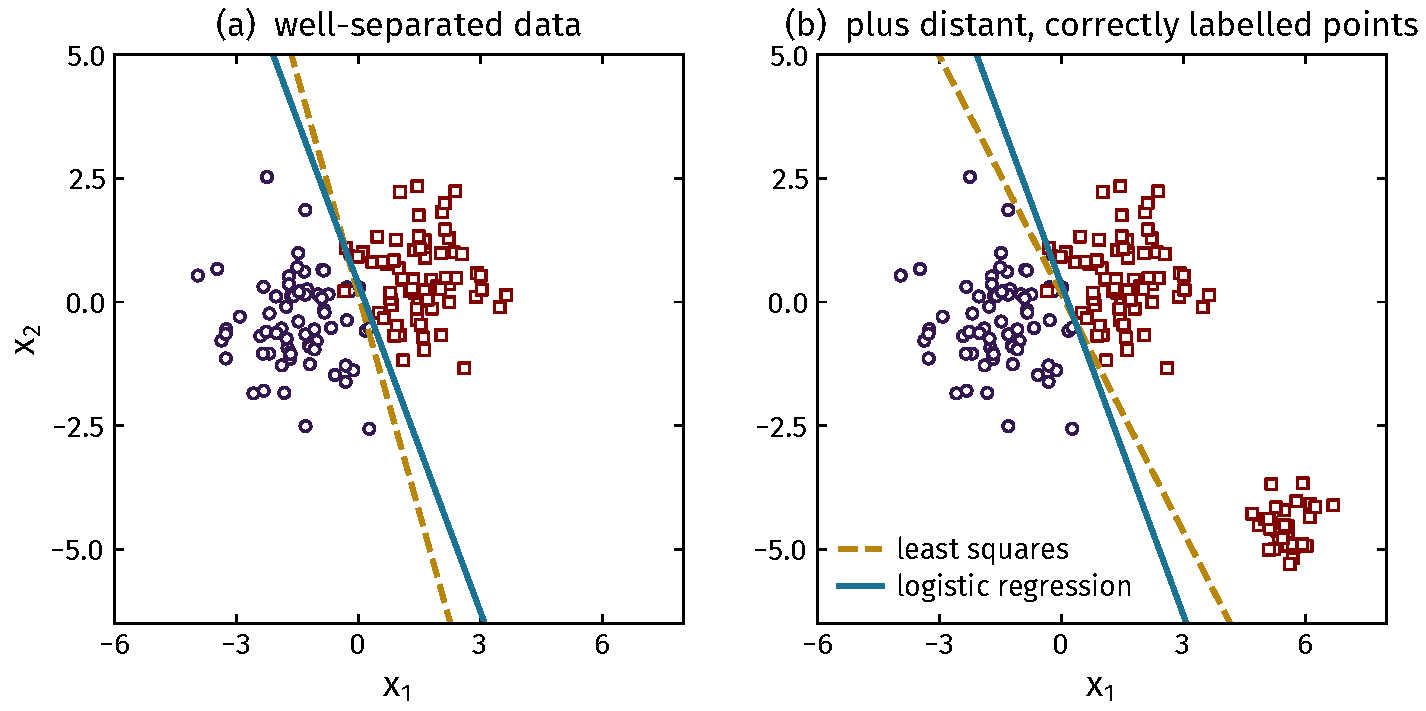
\includegraphics[height=0.40\textheight]{lsq_vs_logistic}
  \end{center}
  \figcap[0.95]{The same two classes, fitted twice. Dashed amber:
  least squares on $0/1$ targets. Solid turquoise: logistic
  regression.}
  \vspace{-0.1em}
  {\footnotesize
  \begin{itemize}\setlength{\itemsep}{1pt}
    \item Distant but \emph{correctly classified} points drag the
          least-squares boundary --- they are penalised for being
          \alert{``too right''}
    \item Squared error is the wrong error for targets in
          $\{0,1\}$; we need one built for \alert{probabilities}
  \end{itemize}}
\end{frame}

\begin{frame}{Where the sigmoid comes from}
  \begin{theorem}[Gaussian classes give a logistic posterior]
    {\small Let $p(\mathbf{x}\mid\mathcal{C}_k)
    =\mathcal{N}(\mathbf{x}\mid\bm\mu_k,\bm\Sigma)$ with a
    \alert{shared} covariance $\bm\Sigma$. Then
    \[
      p(\mathcal{C}_2\mid\mathbf{x})
      = \sigma\big(\mathbf{w}^{\!\top}\mathbf{x}+w_0\big),
      \qquad
      \mathbf{w}=\bm\Sigma^{-1}(\bm\mu_2-\bm\mu_1).
    \]}
  \end{theorem}
  \vspace{0.1em}
  {\footnotesize
  \begin{itemize}\setlength{\itemsep}{1pt}
    \item \focus{1}{By Bayes,
          $p(\mathcal{C}_2\mid\mathbf{x})=\sigma(a)$ where $a$ is
          the \alert{log-odds}
          $a=\ln\dfrac{p(\mathbf{x}\mid\mathcal{C}_2)
          p(\mathcal{C}_2)}{p(\mathbf{x}\mid\mathcal{C}_1)
          p(\mathcal{C}_1)}$}
    \item \focus{2}{Substitute the two Gaussians. The quadratic
          terms $-\tfrac12\mathbf{x}^{\!\top}\bm\Sigma^{-1}
          \mathbf{x}$ are \emph{identical} and cancel --- this is
          exactly where the shared $\bm\Sigma$ is used}
    \item \focus{3}{What survives is linear in $\mathbf{x}$:
          $a=(\bm\mu_2-\bm\mu_1)^{\!\top}\bm\Sigma^{-1}\mathbf{x}
          + w_0$ \hfill $\square$}
    \item \focus{4}{Drop the shared-covariance assumption and the
          quadratic terms remain: the boundary becomes a
          \alert{quadratic} surface}
  \end{itemize}}
\end{frame}

\begin{frame}{The sigmoid, seen in the data}
  \begin{center}
    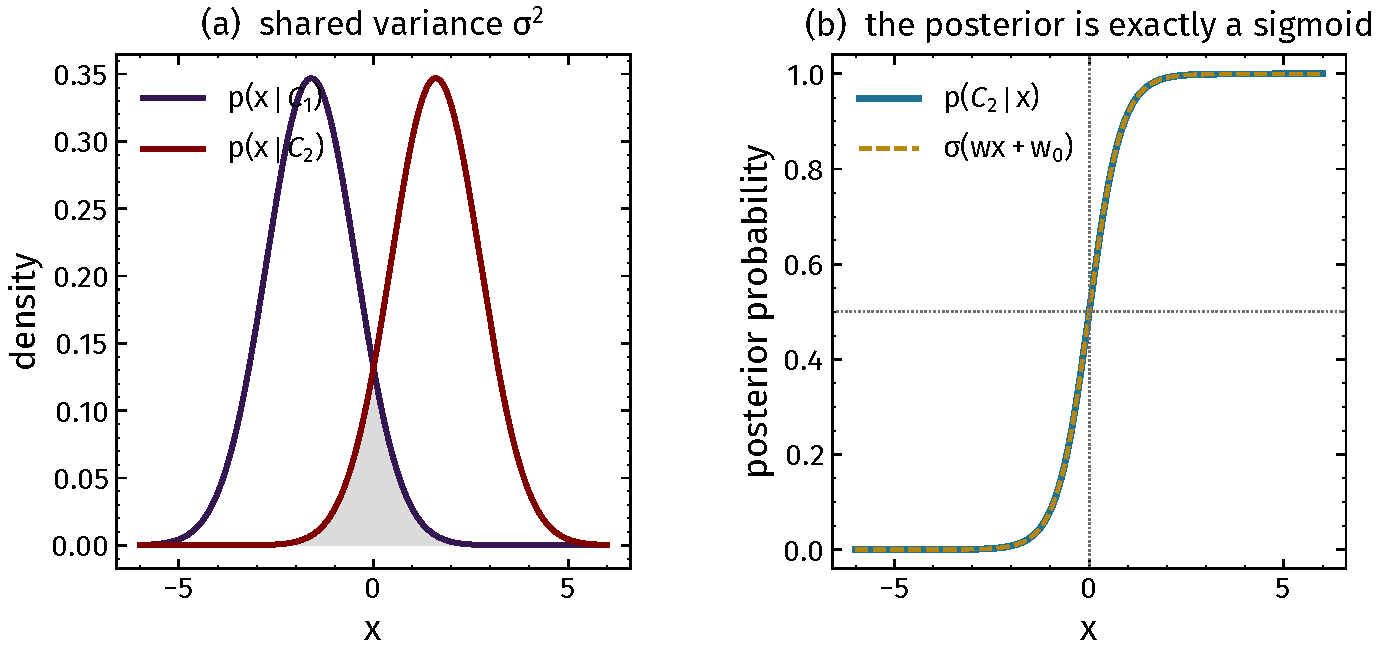
\includegraphics[height=0.435\textheight]{gaussian_posterior}
  \end{center}
  \figcap[0.95]{(a) two Gaussian class-conditionals sharing one
  variance; shaded is their overlap. (b) the exact posterior
  $p(\mathcal{C}_2\mid x)$ in turquoise, with $\sigma(wx+w_0)$
  from the theorem dashed on top --- the two coincide.}
  \vspace{0.1em}
  \begin{redhighlight}
    {\footnotesize The sigmoid is the \alert{natural form of a
    posterior probability}, not an arbitrary squashing choice.}
  \end{redhighlight}
\end{frame}

% =====================================================================
\section{The Maximum-Likelihood Principle}
% =====================================================================

\begin{frame}{Where the error function comes from}
  \vspace{0.2em}
  Rather than choosing an error function by hand, we \alert{derive}
  it. The network predicts the parameters of a probability
  distribution over the output:
  \vfill
  \begin{enumerate}\setlength{\itemsep}{4pt}
    \item Choose a distribution $p(y\mid\cdot)$ suited to the
          \alert{domain of $y$}
    \item Let the network predict its parameters
    \item Train by minimising the \alert{negative log-likelihood}
  \end{enumerate}
  \vfill
  \[
    \hat{\mathbf{w}} = \operatorname*{arg\,min}_{\mathbf{w}}
    \Big[-\sum_{n=1}^{N}
    \ln p\big(y_n \mid \hat y(\mathbf{x}_n,\mathbf{w})\big)\Big]
  \]
  \vfill
  {\footnotesize
  \begin{itemize}\setlength{\itemsep}{2pt}
    \item The logarithm turns products of small numbers into sums,
          and does not move the maximum
    \item Inference: report the \alert{peak} of the predicted
          distribution
  \end{itemize}}
\end{frame}

\begin{frame}{You already know one instance}
  \begin{columns}[T, onlytextwidth]
    \begin{column}{0.54\textwidth}
      \centering
      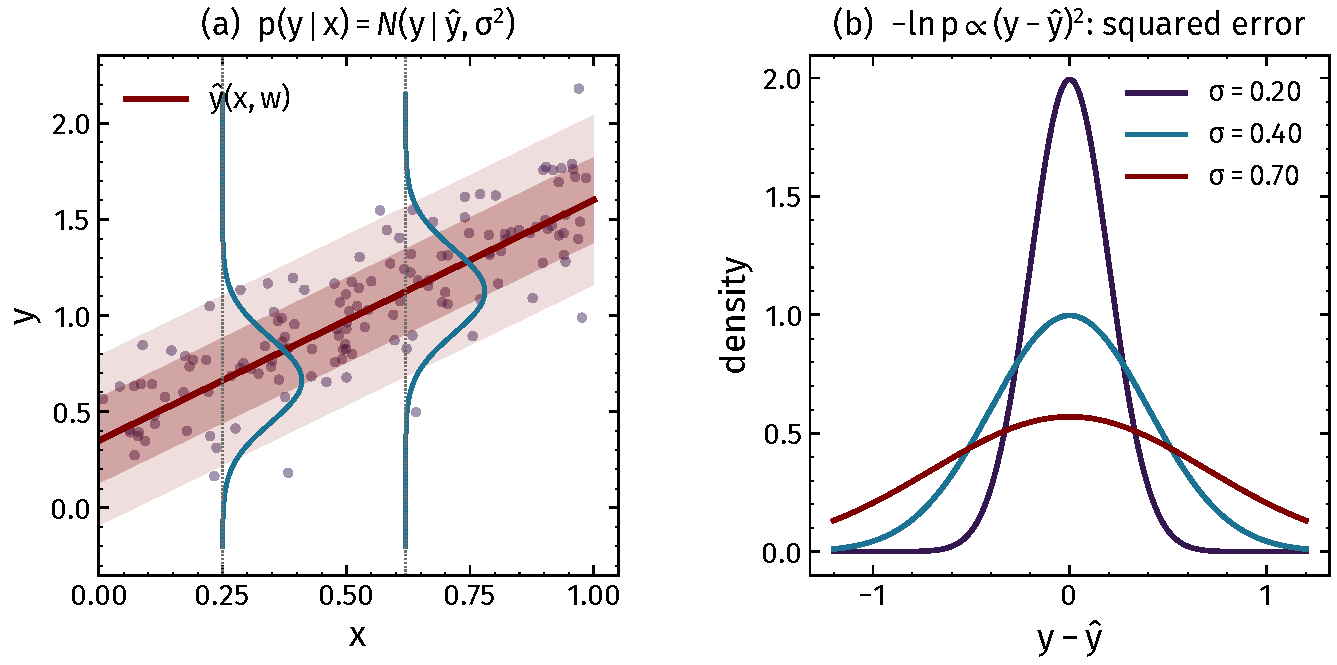
\includegraphics[height=0.44\textheight]{gaussian_ml}
      \\[0.1em]
      \figsource{(a) the model predicts the \emph{mean} of a
      Gaussian at each $x$. (b) its negative log density is a
      parabola in $y-\hat y$.}
    \end{column}
    \hfill
    \begin{column}{0.42\textwidth}
      \vspace{0.5em}
      {\small Class 5, restated in this framework:}
      \vspace{0.3em}
      {\small
      \begin{itemize}\setlength{\itemsep}{5pt}
        \item Domain $y\in\mathbb{R}$ $\to$ choose a
              \alert{Gaussian}
        \item The network predicts its mean $\hat y$
        \item $-\ln p = \dfrac{(y-\hat y)^2}{2\sigma^2}
              + \text{const}$ $\to$ \alert{squared error}
      \end{itemize}}
    \end{column}
  \end{columns}
  \mlparallel{Gaussian noise $\to$ squared error}
             {today: Bernoulli $\to$ cross-entropy, same construction}
\end{frame}

% =====================================================================
\section{Binary Classification}
% =====================================================================

\begin{frame}{Step 1: the Bernoulli distribution}
  \vspace{-0.1em}
  Domain $y\in\{0,1\}$; one parameter, taken to be the prediction:
  \[
    p(y\mid\hat y) = \hat y^{\,y}\,(1-\hat y)^{1-y},
    \qquad \hat y\in[0,1]
  \]
  \vspace{-0.7em}
  \begin{center}
    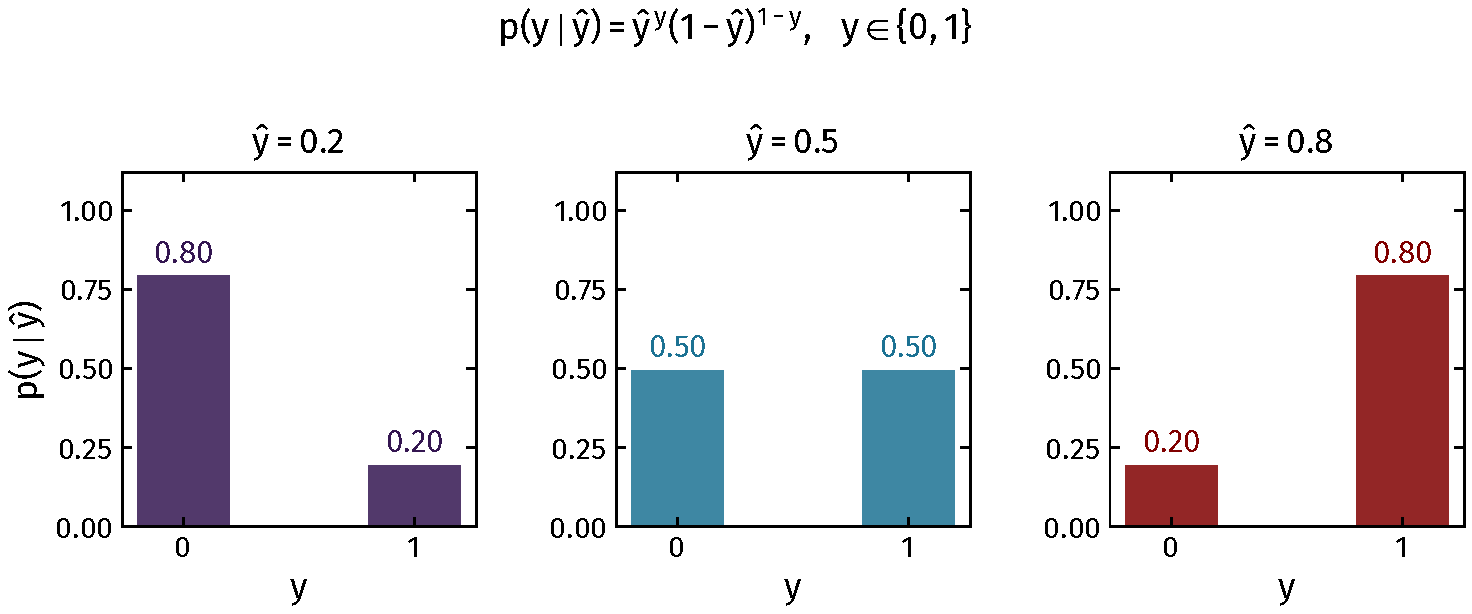
\includegraphics[height=0.365\textheight]{bernoulli}
  \end{center}
  \vspace{-0.3em}
  \figcap[0.97]{The whole distribution is one number --- so the
  network must output a value in $[0,1]$, while the pre-activation
  $a$ is an \alert{arbitrary real number}.}
\end{frame}

\begin{frame}{Step 2: the logistic sigmoid}
  \begin{columns}[T, onlytextwidth]
    \begin{column}{0.44\textwidth}
      \vspace{0.3em}
      {\small Map $\mathbb{R}$ onto $(0,1)$
      (B\&B, 2024, Eq.~5.42):}
      \[
        \hat y = \sigma(a) = \frac{1}{1+\exp(-a)}
      \]
      \vspace{0.6em}
      {\small
      \begin{itemize}\setlength{\itemsep}{5pt}
        \item $a$ is the \alert{log-odds}:
              $a=\ln\dfrac{\hat y}{1-\hat y}$
        \item $a/\lVert\mathbf{w}\rVert$ was the distance to the
              boundary --- distance becomes confidence
      \end{itemize}}
    \end{column}
    \hfill
    \begin{column}{0.52\textwidth}
      \centering
      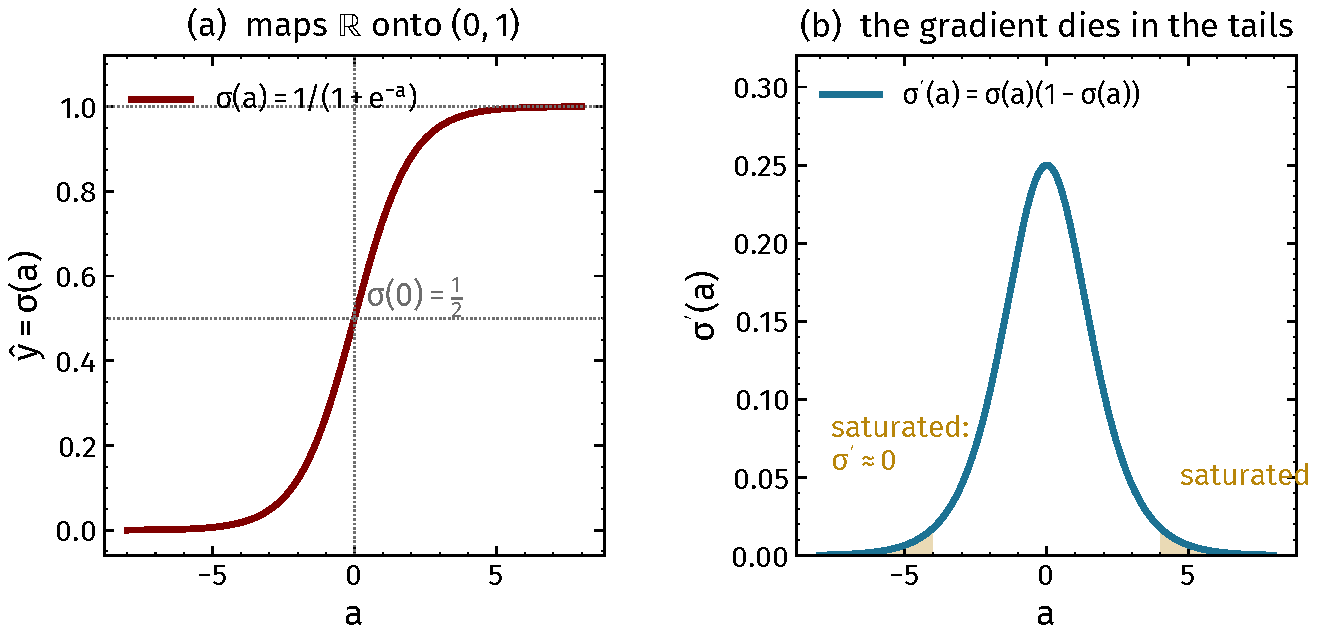
\includegraphics[height=0.345\textheight]{sigmoid}
      \\[0.1em]
      \figsource{(a) the sigmoid. (b) its derivative, which all
      but vanishes once $|a|\gtrsim 4$.}
    \end{column}
  \end{columns}
  \mlparallel{$\sigma(\mathbf{w}^{\!\top}
              \boldsymbol\phi(\mathbf{x}))$}
             {the same sigmoid, on a learned-feature read-out}
\end{frame}

\begin{frame}{Properties we will need}
  \begin{propx}[The logistic sigmoid]
    {\small For all $a\in\mathbb{R}$:
    \[
      \text{(i) } \sigma(-a)=1-\sigma(a),
      \quad
      \text{(ii) } \sigma'(a)=\sigma(a)\big(1-\sigma(a)\big),
      \quad
      \text{(iii) } \sigma^{-1}(u)=\ln\frac{u}{1-u}.
    \]}
  \end{propx}
  \vspace{-0.1em}
  {\scriptsize
  \begin{itemize}\setlength{\itemsep}{2pt}
    \item \focus{1}{(i) $\sigma(-a)=\dfrac{1}{1+e^{a}}
          =\dfrac{e^{-a}}{e^{-a}+1}
          =1-\dfrac{1}{1+e^{-a}}$}
    \item \focus{2}{(ii) Differentiate:
          $\sigma'(a)=\dfrac{e^{-a}}{(1+e^{-a})^{2}}
          =\dfrac{1}{1+e^{-a}}\cdot\dfrac{e^{-a}}{1+e^{-a}}
          =\sigma(a)\big(1-\sigma(a)\big)$}
    \item \focus{3}{(iii) Solve $u=1/(1+e^{-a})$:
          $e^{-a}=(1-u)/u$, hence $a=\ln\frac{u}{1-u}$
          \hfill $\square$}
  \end{itemize}}
  \vspace{-0.2em}
  \begin{redhighlight}
    {\scriptsize (ii) is the identity that makes the cross-entropy
    gradient collapse to something very simple; (iii) says the
    pre-activation \emph{is} the log-odds.}
  \end{redhighlight}
\end{frame}

\begin{frame}{Step 3: binary cross-entropy}
  \vspace{0.2em}
  Negative log-likelihood of the Bernoulli model over $N$
  independent examples (B\&B, 2024, Eq.~5.74):
  \[
    E(\mathbf{w}) = -\sum_{n=1}^{N}\Big[
      y_n\ln \hat y_n + (1-y_n)\ln(1-\hat y_n)\Big],
    \qquad \hat y_n=\sigma(a_n)
  \]
  \vfill
  {\small
  \begin{itemize}\setlength{\itemsep}{5pt}
    \item Only one term is active per example: $y_n{=}1$ charges
          $-\ln\hat y_n$, and $y_n{=}0$ charges
          $-\ln(1-\hat y_n)$
    \item Both are zero for a perfect prediction and diverge for a
          confident mistake
  \end{itemize}}
  \mlparallel{logistic regression: convex in $\mathbf{w}$}
             {same error, non-convex once a network is inside}
\end{frame}

\begin{frame}{The gradient is as simple as it could be}
  \begin{theorem}[Cross-entropy gradient]
    {\small With $\hat y_n=\sigma(a_n)$ and $E$ the binary
    cross-entropy,
    \[
      \frac{\partial E}{\partial a_n} = \hat y_n - y_n,
      \qquad\text{so}\qquad
      \nabla_{\mathbf{w}} E
      = \sum_{n=1}^{N}(\hat y_n - y_n)\,\boldsymbol\phi_n
      \tag{B\&B 5.75}
    \]
    for a linear model $a_n=\mathbf{w}^{\!\top}
    \boldsymbol\phi_n$.}
  \end{theorem}
  \vspace{0.1em}
  {\footnotesize
  \begin{itemize}\setlength{\itemsep}{2pt}
    \item \focus{1}{$\dfrac{\partial E}{\partial\hat y_n}
          = -\dfrac{y_n}{\hat y_n}
          + \dfrac{1-y_n}{1-\hat y_n}
          = \dfrac{\hat y_n-y_n}{\hat y_n(1-\hat y_n)}$}
    \item \focus{2}{By Proposition (ii),
          $\dfrac{\partial\hat y_n}{\partial a_n}
          =\hat y_n(1-\hat y_n)$}
    \item \focus{3}{Chain rule: the two factors
          $\hat y_n(1-\hat y_n)$ \alert{cancel exactly}, leaving
          $\partial E/\partial a_n=\hat y_n-y_n$}
    \item \focus{4}{Finally
          $\partial a_n/\partial\mathbf{w}=\boldsymbol\phi_n$
          gives the sum \hfill $\square$}
  \end{itemize}}
\end{frame}

\begin{frame}{The binary model, end to end}
  \begin{center}
    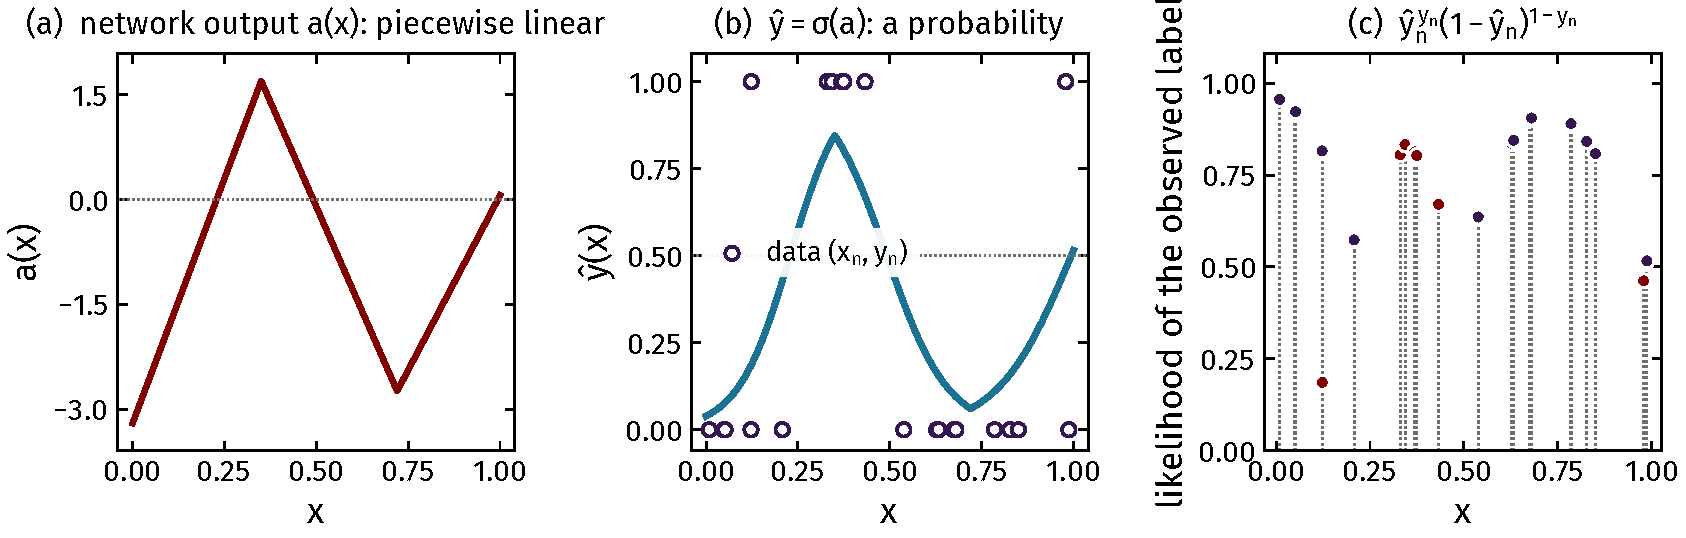
\includegraphics[height=0.475\textheight]{binary_model}
  \end{center}
  \figcap[0.96]{(a) the network output $a(x)$ --- still piecewise
  linear, exactly as in Class 5. (b) after the sigmoid it is a
  probability, with the observed labels overlaid. (c) the
  likelihood each point assigns to the label it actually carries;
  training pushes all of these upwards.}
\end{frame}

\begin{frame}{Why not squared error on probabilities?}
  \begin{propx}[Squared error saturates]
    {\small With a sigmoid output,
    $\dfrac{\partial E_{\mathrm{SSE}}}{\partial a}
    = (\hat y-y)\,\sigma'(a)$, whereas
    $\dfrac{\partial E_{\mathrm{CE}}}{\partial a}=\hat y-y$.
    Since $\sigma'(a)\to 0$ as $|a|\to\infty$, the squared-error
    gradient vanishes even when the prediction is confidently
    wrong.}
  \end{propx}
  \vspace{-0.1em}
  \begin{center}
    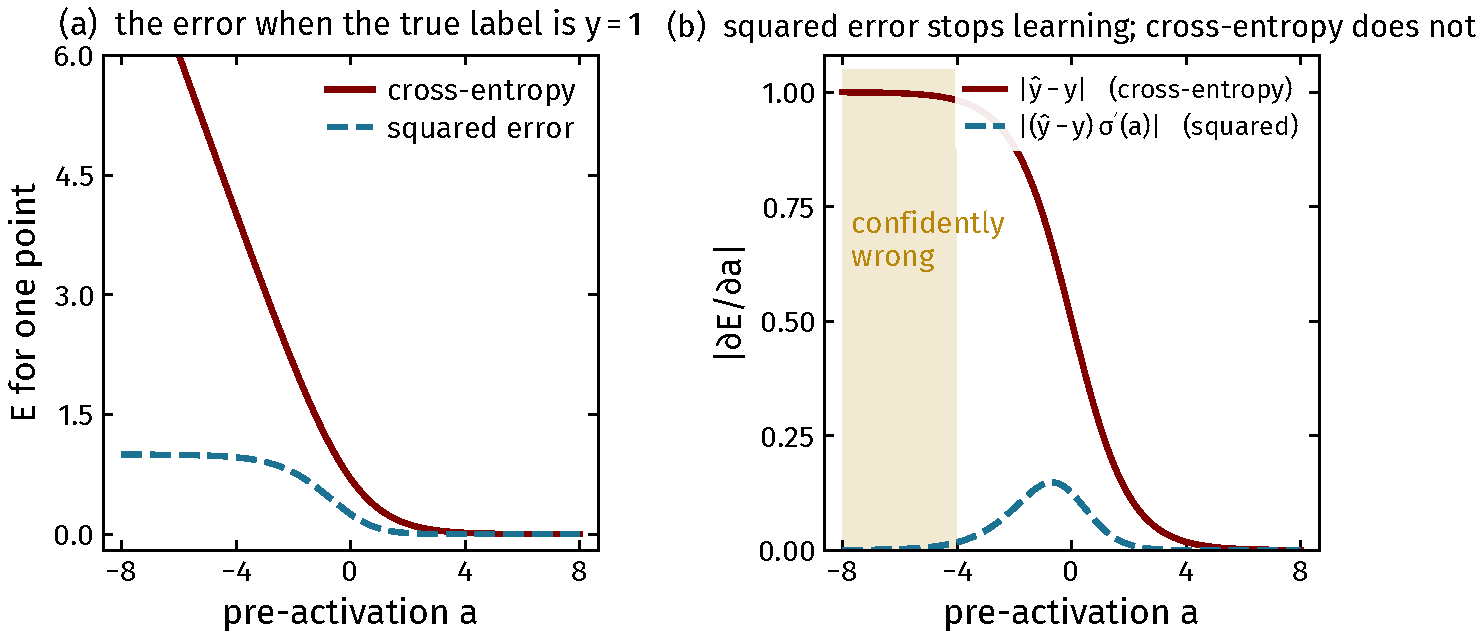
\includegraphics[height=0.275\textheight]{saturation}
  \end{center}
  \figcap[0.94]{True label $y=1$. Shaded: confidently wrong. The
  squared-error gradient dies there; cross-entropy stays at full
  strength.}
\end{frame}

% =====================================================================
\section{Multi-class Classification}
% =====================================================================

\begin{frame}{Step 1: the categorical distribution}
  \vspace{-0.1em}
  Domain $y\in\{1,\dots,K\}$, one-hot encoded; $K$ parameters:
  \[
    p(y=k) = \hat y_k,
    \qquad
    \hat y_k \ge 0,
    \qquad
    \textstyle\sum_{k=1}^{K} \hat y_k = 1
  \]
  \vspace{-0.7em}
  \begin{center}
    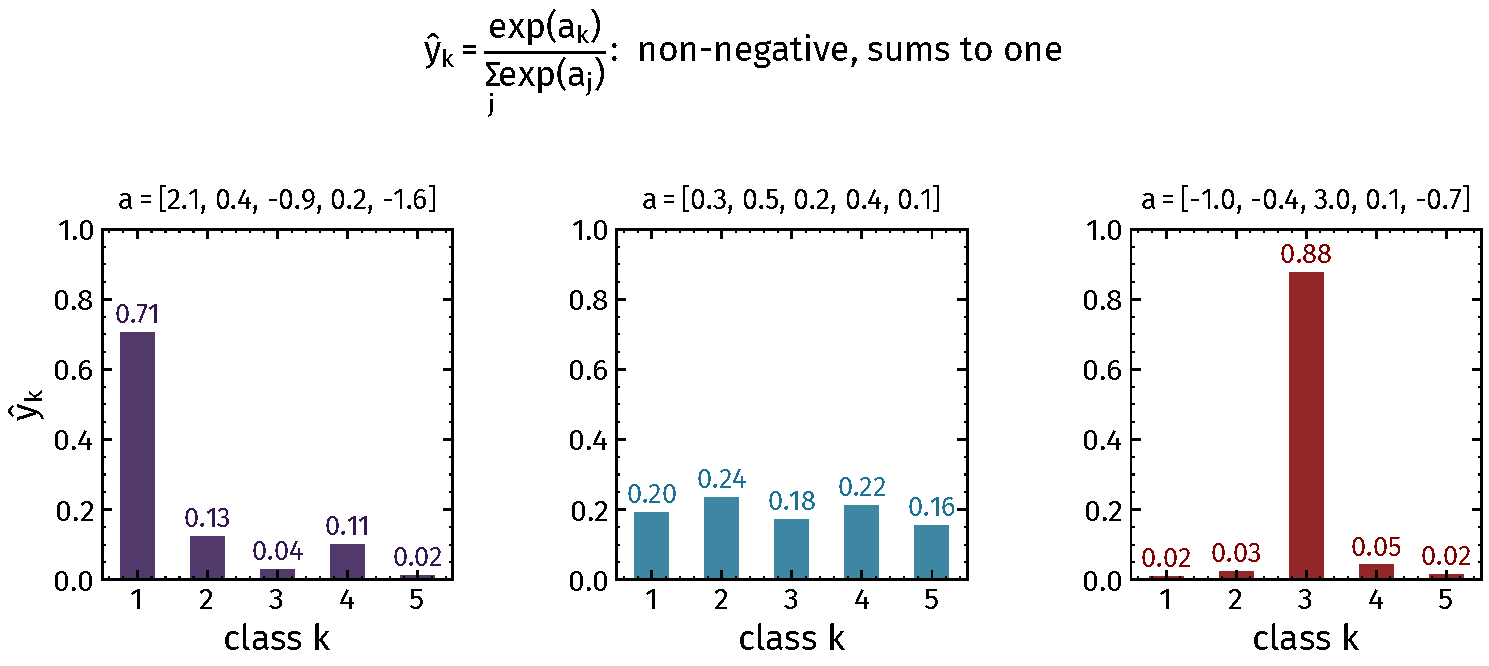
\includegraphics[height=0.395\textheight]{categorical}
  \end{center}
  \vspace{-0.3em}
  \figcap[0.97]{Three sets of pre-activations and the distributions
  they produce; the raw $a_1,\dots,a_K$ are unconstrained.}
\end{frame}

\begin{frame}{Step 2: softmax}
  \vspace{0.2em}
  Normalise the exponentiated pre-activations
  (B\&B, 2024, Eqs.~5.76--5.77):
  \[
    \hat y_k = \mathrm{softmax}_k(\mathbf{a})
    = \frac{\exp(a_k)}{\sum_{j=1}^{K}\exp(a_j)}
  \]
  \vfill
  \begin{propx}[Softmax]
    {\small (i) $\hat y_k>0$ and $\sum_k\hat y_k=1$.
    (ii) \alert{Shift invariance}:
    $\mathrm{softmax}(\mathbf{a}+c\mathbf{1})
    =\mathrm{softmax}(\mathbf{a})$ for any $c$.
    (iii) For $K=2$ it \alert{is} the sigmoid:
    $\hat y_1=\sigma(a_1-a_2)$.}
  \end{propx}
  \vspace{0.1em}
  {\scriptsize
  \emph{Proof.} (i) is immediate. (ii) multiplies numerator and
  denominator by $e^{c}$. (iii)
  $\frac{e^{a_1}}{e^{a_1}+e^{a_2}}=\frac{1}{1+e^{-(a_1-a_2)}}$.
  \hfill$\square$}
  \vspace{0.3em}

  {\scriptsize (ii) is what makes the computation numerically safe:
  subtract $\max_k a_k$ before exponentiating.}
  \vspace{0.45em}
  \mlparallel{multinomial logistic regression}
             {softmax on $K$ learned-feature read-outs}
\end{frame}

\begin{frame}{The softmax Jacobian}
  \begin{lemmax}[Derivative of softmax]
    {\small For $\hat y_k=\mathrm{softmax}_k(\mathbf{a})$,
    \[
      \frac{\partial \hat y_k}{\partial a_j}
      = \hat y_k\,\big(\delta_{kj} - \hat y_j\big),
      \qquad
      \delta_{kj}=\begin{cases}1 & k=j\\ 0 & k\ne j.\end{cases}
    \]}
  \end{lemmax}
  \vspace{0.1em}
  {\footnotesize
  \begin{itemize}\setlength{\itemsep}{2pt}
    \item \focus{1}{Write $\hat y_k = e^{a_k}/S$ with
          $S=\sum_j e^{a_j}$, so
          $\partial S/\partial a_j = e^{a_j}$}
    \item \focus{2}{Quotient rule:
          $\dfrac{\partial\hat y_k}{\partial a_j}
          = \dfrac{\delta_{kj}\,e^{a_k}S - e^{a_k}e^{a_j}}{S^{2}}$}
    \item \focus{3}{Divide through and recognise
          $e^{a_k}/S=\hat y_k$, $e^{a_j}/S=\hat y_j$:
          $\;=\hat y_k\delta_{kj}-\hat y_k\hat y_j$
          \hfill $\square$}
    \item \focus{4}{Check $K=2$: this gives
          $\hat y_1(1-\hat y_1)$ --- the sigmoid derivative
          again}
  \end{itemize}}
\end{frame}

\begin{frame}{Step 3: multi-class cross-entropy}
  \begin{theorem}[Cross-entropy and its gradient]
    {\small With one-hot targets $y_{nk}$ and
    $\hat y_{nk}=\mathrm{softmax}_k(\mathbf{a}_n)$,
    \[
      E(\mathbf{w}) = -\sum_{n=1}^{N}\sum_{k=1}^{K}
      y_{nk}\,\ln \hat y_{nk},
      \qquad
      \frac{\partial E}{\partial a_{nk}} = \hat y_{nk}-y_{nk}.
      \tag{B\&B 5.80--5.81}
    \]}
  \end{theorem}
  \vspace{0.1em}
  {\footnotesize
  \begin{itemize}\setlength{\itemsep}{1pt}
    \item \focus{1}{$\dfrac{\partial E_n}{\partial a_{nk}}
          = -\sum_{c} \dfrac{y_{nc}}{\hat y_{nc}}\,
          \dfrac{\partial \hat y_{nc}}{\partial a_{nk}}$}
    \item \focus{2}{Insert the Lemma:
          $= -\sum_{c} \dfrac{y_{nc}}{\hat y_{nc}}\,
          \hat y_{nc}(\delta_{ck}-\hat y_{nk})
          = -\sum_{c} y_{nc}(\delta_{ck}-\hat y_{nk})$}
    \item \focus{3}{Split:
          $= -y_{nk} + \hat y_{nk}\sum_{c} y_{nc}
          = \hat y_{nk}-y_{nk}$, since
          $\sum_c y_{nc}=1$ \hfill $\square$}
  \end{itemize}}
  \vspace{-0.2em}
  \begin{redhighlight}
    {\scriptsize Regression, binary, multi-class: the output-layer
    gradient is \alert{$\hat y - y$} every time.}
  \end{redhighlight}
\end{frame}

\begin{frame}{Softmax posteriors over the input space}
  \begin{center}
    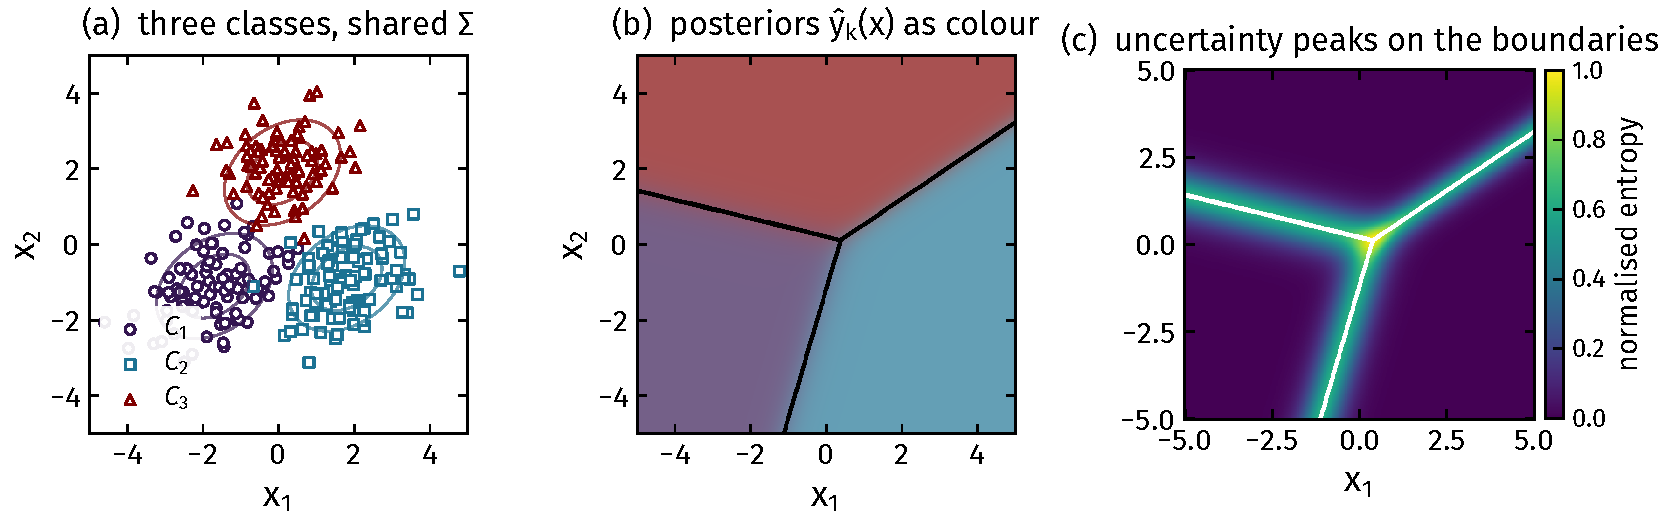
\includegraphics[height=0.51\textheight]{softmax_posteriors}
  \end{center}
  \figcap[0.96]{(a) three Gaussian classes with a shared
  covariance. (b) the posteriors as a colour blend, decision
  boundaries in black --- each region is where one class
  dominates. (c) the entropy of the posterior: the model is
  uncertain exactly along the boundaries, and most uncertain where
  all three meet.}
\end{frame}

\begin{frame}{The multi-class model on a scalar input}
  \begin{center}
    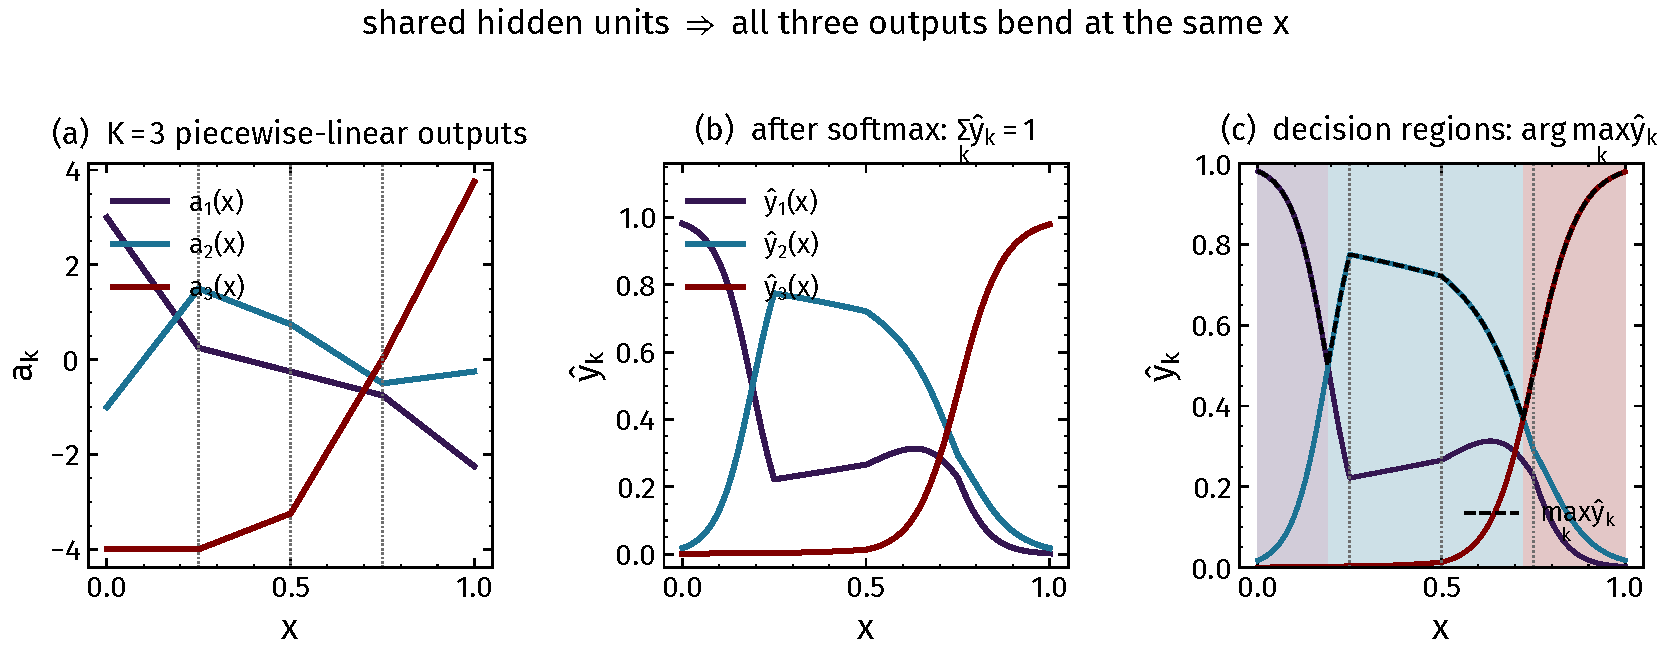
\includegraphics[height=0.50\textheight]{multiclass_model}
  \end{center}
  \figcap[0.96]{(a) $K=3$ pre-activations from one shared hidden
  layer, so they bend at the same $x$ (dotted). (b) after softmax
  they are non-negative and sum to one. (c) the decision regions
  $\arg\max_k\hat y_k$, shaded; the dashed line is the winning
  probability, which dips where the regions meet.}
\end{frame}

% =====================================================================
\section{The Bigger Picture}
% =====================================================================

\begin{frame}{One principle, any output type}
  \begin{center}
    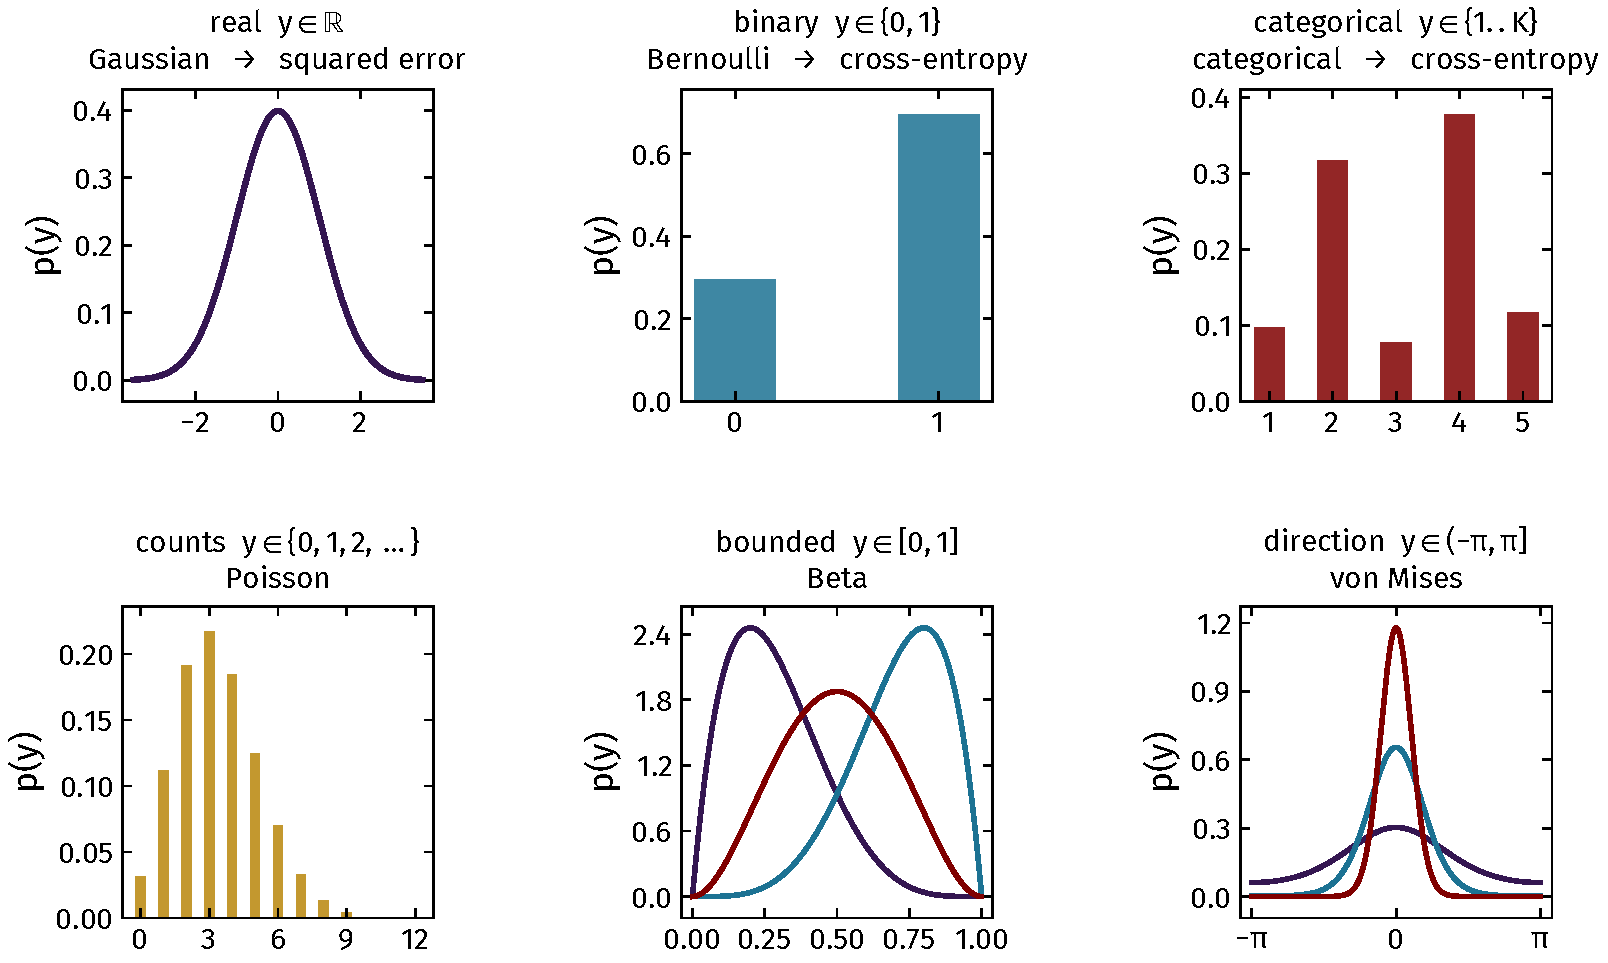
\includegraphics[height=0.585\textheight]{output_distributions}
  \end{center}
  \figcap[0.94]{Match the distribution to the domain of $y$ and the
  error function follows. Counts, bounded values and directions each
  have their own natural choice.}
\end{frame}

\begin{frame}{Cross-entropy: the second view}
  \begin{theorem}[Maximum likelihood $=$ minimum KL divergence]
    {\small Let $q$ be the empirical distribution of the data and
    $p$ the model. Then
    \[
      -\frac1N\sum_{n}\ln p(y_n)
      \;=\; H(q,p)
      \;=\; \underbrace{H(q)}_{\text{fixed by the data}}
      + \mathrm{KL}(q\,\|\,p),
    \]
    so minimising the negative log-likelihood is exactly
    minimising $\mathrm{KL}(q\|p)$.}
  \end{theorem}
  \vspace{0.1em}
  {\footnotesize
  \emph{Proof.} $H(q,p)=-\sum_y q(y)\ln p(y)$; with $q$ the
  empirical distribution this average \emph{is} the mean negative
  log-likelihood. Add and subtract $\sum_y q\ln q$ to get
  $H(q,p) = H(q) + \sum_y q\ln(q/p)$. The first term does not
  involve the model, and $\mathrm{KL}\ge 0$ with equality only
  when $p=q$. \hfill$\square$}
  \vspace{-0.2em}
  \begin{redhighlight}
    {\scriptsize Hence the name \alert{cross-entropy}: it is
    $H(q,p)$, the cost of coding data from $q$ using the model
    $p$.}
  \end{redhighlight}
\end{frame}

\begin{frame}{The same statement, drawn}
  \begin{center}
    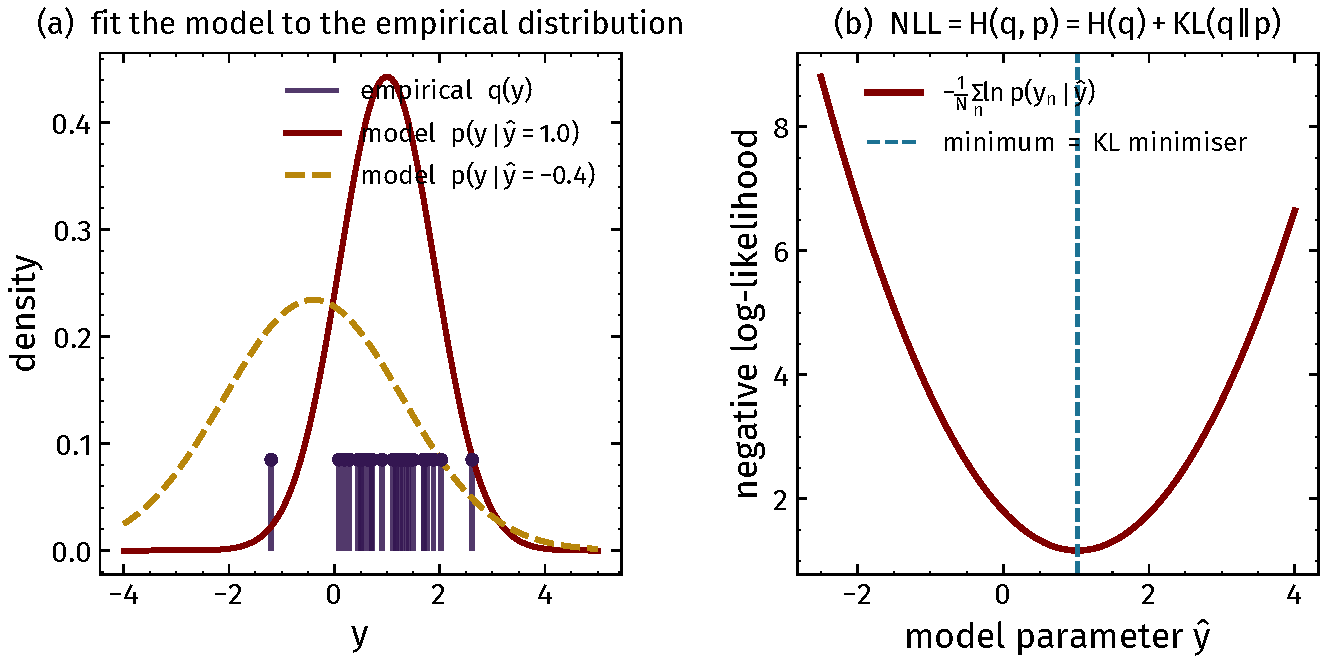
\includegraphics[height=0.50\textheight]{cross_entropy_kl}
  \end{center}
  \figcap[0.95]{(a) the empirical distribution (spikes at the
  observed values) and two candidate models; the dashed one places
  little mass where the data actually are. (b) the negative
  log-likelihood as the model parameter varies --- its minimum is
  the point of smallest KL divergence.}
\end{frame}

\begin{frame}{Fixed features vs.\ learned features, again}
  \begin{center}
    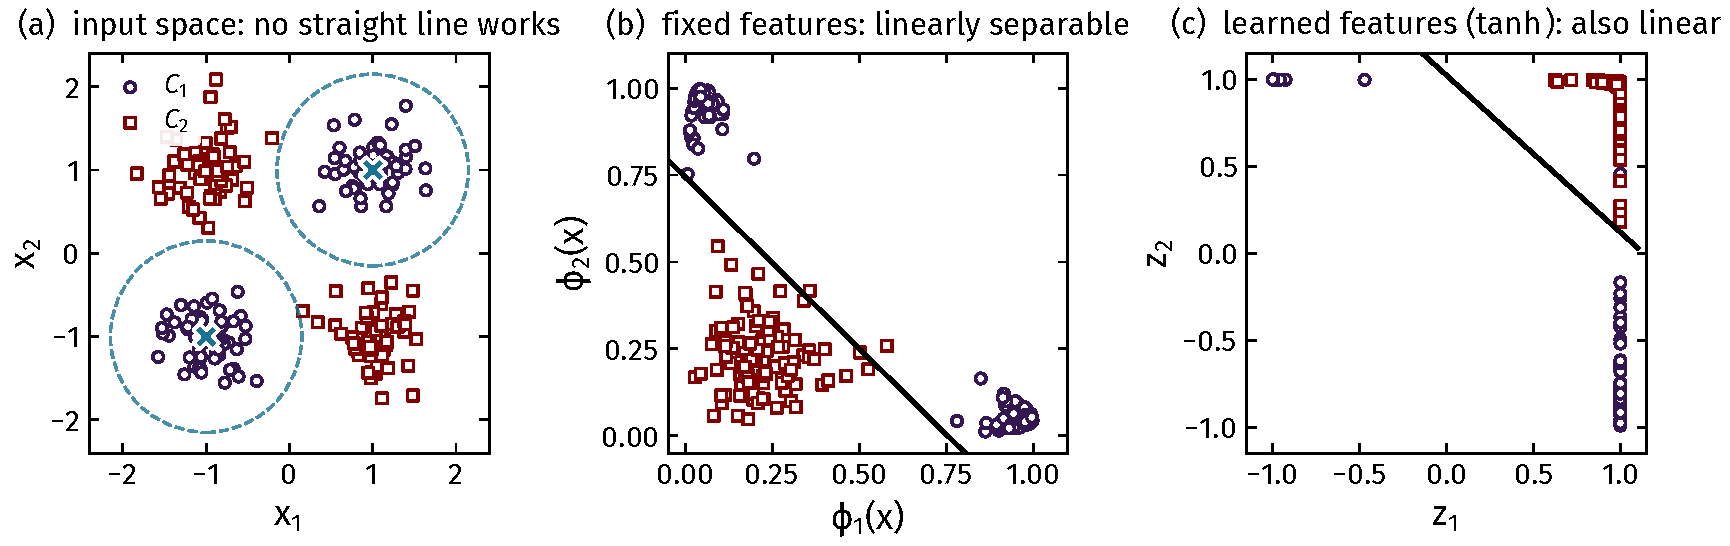
\includegraphics[height=0.42\textheight]{feature_space}
  \end{center}
  \figcap[0.96]{(a) four clusters in XOR arrangement: no straight
  line separates them. (b) mapped by two \emph{fixed} Gaussian
  basis functions centred at the crosses --- now a single line
  does it. (c) mapped by the two \emph{learned} $\tanh$ hidden
  units of a trained network: also linearly separable, but the
  network chose the map itself.}
  \mlparallel{fixed $\boldsymbol\phi$, chosen to linearise the
              problem}
             {a network \emph{learns} a map that linearises it}
\end{frame}

\begin{frame}{Output activations: the complete table}
  \centering
  \renewcommand{\arraystretch}{1.3}
  {\small
  \begin{tabular}{p{0.17\textwidth} p{0.17\textwidth}
                  p{0.22\textwidth} p{0.28\textwidth}}
    \textbf{Task} & \textbf{Distribution} &
    \textbf{Output activation} & \textbf{Error}\\
    \hline
    Regression & Gaussian & identity & sum of squares\\
    Binary & Bernoulli & sigmoid $\sigma(a)$ &
      binary cross-entropy\\
    Multi-class & categorical & softmax & cross-entropy\\
    \hline
  \end{tabular}}
  \vspace{0.8em}

  {\small In all three cases the output-layer gradient is
  \alert{$\hat y_n - y_n$}: prediction minus target.}
  \vspace{0.4em}

  \begin{redhighlight}
    {\small Choose the distribution first. The output activation
    and the error function are then \alert{determined}, not
    chosen.}
  \end{redhighlight}
\end{frame}

\begin{frame}{The dictionary (Classes 5--6)}
  \centering
  \renewcommand{\arraystretch}{1.12}
  {\footnotesize
  \begin{tabular}{p{0.17\textwidth} p{0.36\textwidth}
                  p{0.36\textwidth}}
    & \textbf{\color{mlc}Linear/Basis-Function Model}
    & \textbf{\color{nnc}Shallow Neural Network}\\
    \hline
    Features
      & $\phi_j(\mathbf{x})$, fixed
      & $z_j = h(a_j)$, learned\\
    Regression
      & $\mathbf{w}^{\!\top}\boldsymbol{\phi}$; squared error;
        normal equations
      & linear read-out; squared error; gradient descent\\
    Binary
      & $\sigma(\mathbf{w}^{\!\top}\boldsymbol{\phi})$;
        cross-entropy; convex
      & $\sigma(\text{read-out})$; cross-entropy; non-convex\\
    Multi-class
      & softmax; cross-entropy; convex
      & softmax; cross-entropy; non-convex\\
    Boundary
      & hyperplane in a \emph{chosen} feature space
      & hyperplane in a \emph{learned} feature space\\
    \hline
  \end{tabular}}
  \vspace{0.6em}
  \begin{redhighlight}
    Classification is the Class-5 network with a new output
    activation and the error function that matches it.
  \end{redhighlight}
\end{frame}

\begin{frame}{Takeaways}
  \vspace{0.1em}
  {\footnotesize
  \begin{enumerate}\setlength{\itemsep}{2pt}
    \item The error function \alert{follows from a distribution
          over outputs}: pick it to match the domain of $y$,
          predict its parameters, minimise the negative
          log-likelihood
    \item Binary: Bernoulli $\to$ sigmoid $\to$ binary
          cross-entropy. The sigmoid is not a convenience --- for
          Gaussian classes with shared covariance the posterior
          \alert{is} a sigmoid, exactly
    \item Multi-class: categorical $\to$ softmax $\to$
          cross-entropy, and softmax reduces to the sigmoid when
          $K=2$
    \item Every case has output gradient \alert{$\hat y-y$};
          mismatching the error to the distribution reintroduces a
          $\sigma'$ factor and learning stalls
    \item Minimising the negative log-likelihood is minimising a
          \alert{KL divergence} to the empirical distribution
  \end{enumerate}}
  \vspace{0.2em}
  \begin{redhighlight}
    {\footnotesize Class~7: stacking hidden layers ---
    \alert{deep networks}, and why depth buys more than width.}
  \end{redhighlight}
\end{frame}

\begin{frame}{References}
  \footnotesize
  \begin{itemize}\setlength{\itemsep}{3pt}
    \item C.~M.~Bishop \& H.~Bishop. \textit{Deep Learning:
          Foundations and Concepts.} Springer, 2024.
          \S5.1 (discriminant functions and their geometry),
          \S5.2 (decision theory), \S5.3 (probabilistic generative
          models, the logistic posterior), \S5.4 (logistic
          regression, cross-entropy and its gradients),
          \S6.1 (feed-forward networks).
    \item S.~J.~D.~Prince. \textit{Understanding Deep Learning.}
          MIT Press, 2023. Ch.~5 --- deriving the error function
          from a distribution over outputs, and the catalogue of
          output distributions.
    \item All plots generated by \texttt{src/build\_all.py}
          (NumPy, Matplotlib, SciencePlots); one module per figure
          under \texttt{src/figures/}. Notation follows
          \texttt{\_shared/NOTATION.md}.
  \end{itemize}
\end{frame}

\begin{frame}[standout]
  Questions?
\end{frame}

\end{document}
